\documentclass[12pt]{article}

\usepackage[a4paper,top=1cm,bottom=2cm,left=2.1cm,right=2.1cm,marginparwidth=1.75cm]{geometry}
\usepackage{graphicx}
\usepackage{lmodern}
\usepackage{float}
\usepackage{microtype}
\usepackage{amsmath}
\usepackage{amssymb}
\usepackage{tikz}
\usepackage{url}
\usepackage{setspace}
\usepackage[colorlinks=true, allcolors=blue]{hyperref}


\begin{document}
\title{Neural Network - Implementation in Java}
    \author{Daniel K. Ayivon - kdayivon} 
    \date{\today}

    \maketitle

    \begin{abstract}
        This work serves as compedium of machine learning knowledge, in which fundamentals ideas of Linear Algebra, Calculus, and 
        programming paradigms are explored for deeper comprehension.
    \end{abstract}

    \section{Perceptron - Neural Model}
    In machine learning, a perceptron can be broadly defined as an "artifical neuron"—a variable that holds a value.
    \begin{figure}[htbp]
        \centering
        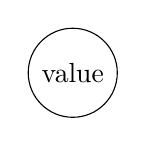
\begin{tikzpicture}
            \node[shape=circle, draw=black] (N) at (0, 0) {value}; 
        \end{tikzpicture}
        \caption{Simple representation of a Perceptron}
        \label{fig:1n}
    \end{figure}
    A \textit{Multi-Layer Perceptron}, 
    or \textit{Neural Network}, is a programming paradigm where each layer of the network is composed of multiple perceptrons, 
    each holding a value, akin to vectors. The network is usually divided into three distinctive but connected parts :
    \begin{itemize}
        \item The input layer - can also be considered as the 0\textsuperscript{th} activation layer. Each perceptron in this 
            layer holds a input—generally a float, given by the training data.
        \item The hidden layer - composed of \textit{n} layers, each perceptron holding the value of a function where the
            parameters is each individual perceptron, weights, and biases of the previous layer.
        \item The output layer - the expected outputs given by the instance of data.
    \end{itemize}
    We can conceptually assume that the hidden layers of a neural network split the inputs into different recognizable patterns,
    which could combine into the expected output.   
    \begin{figure}[H]
        \centering
        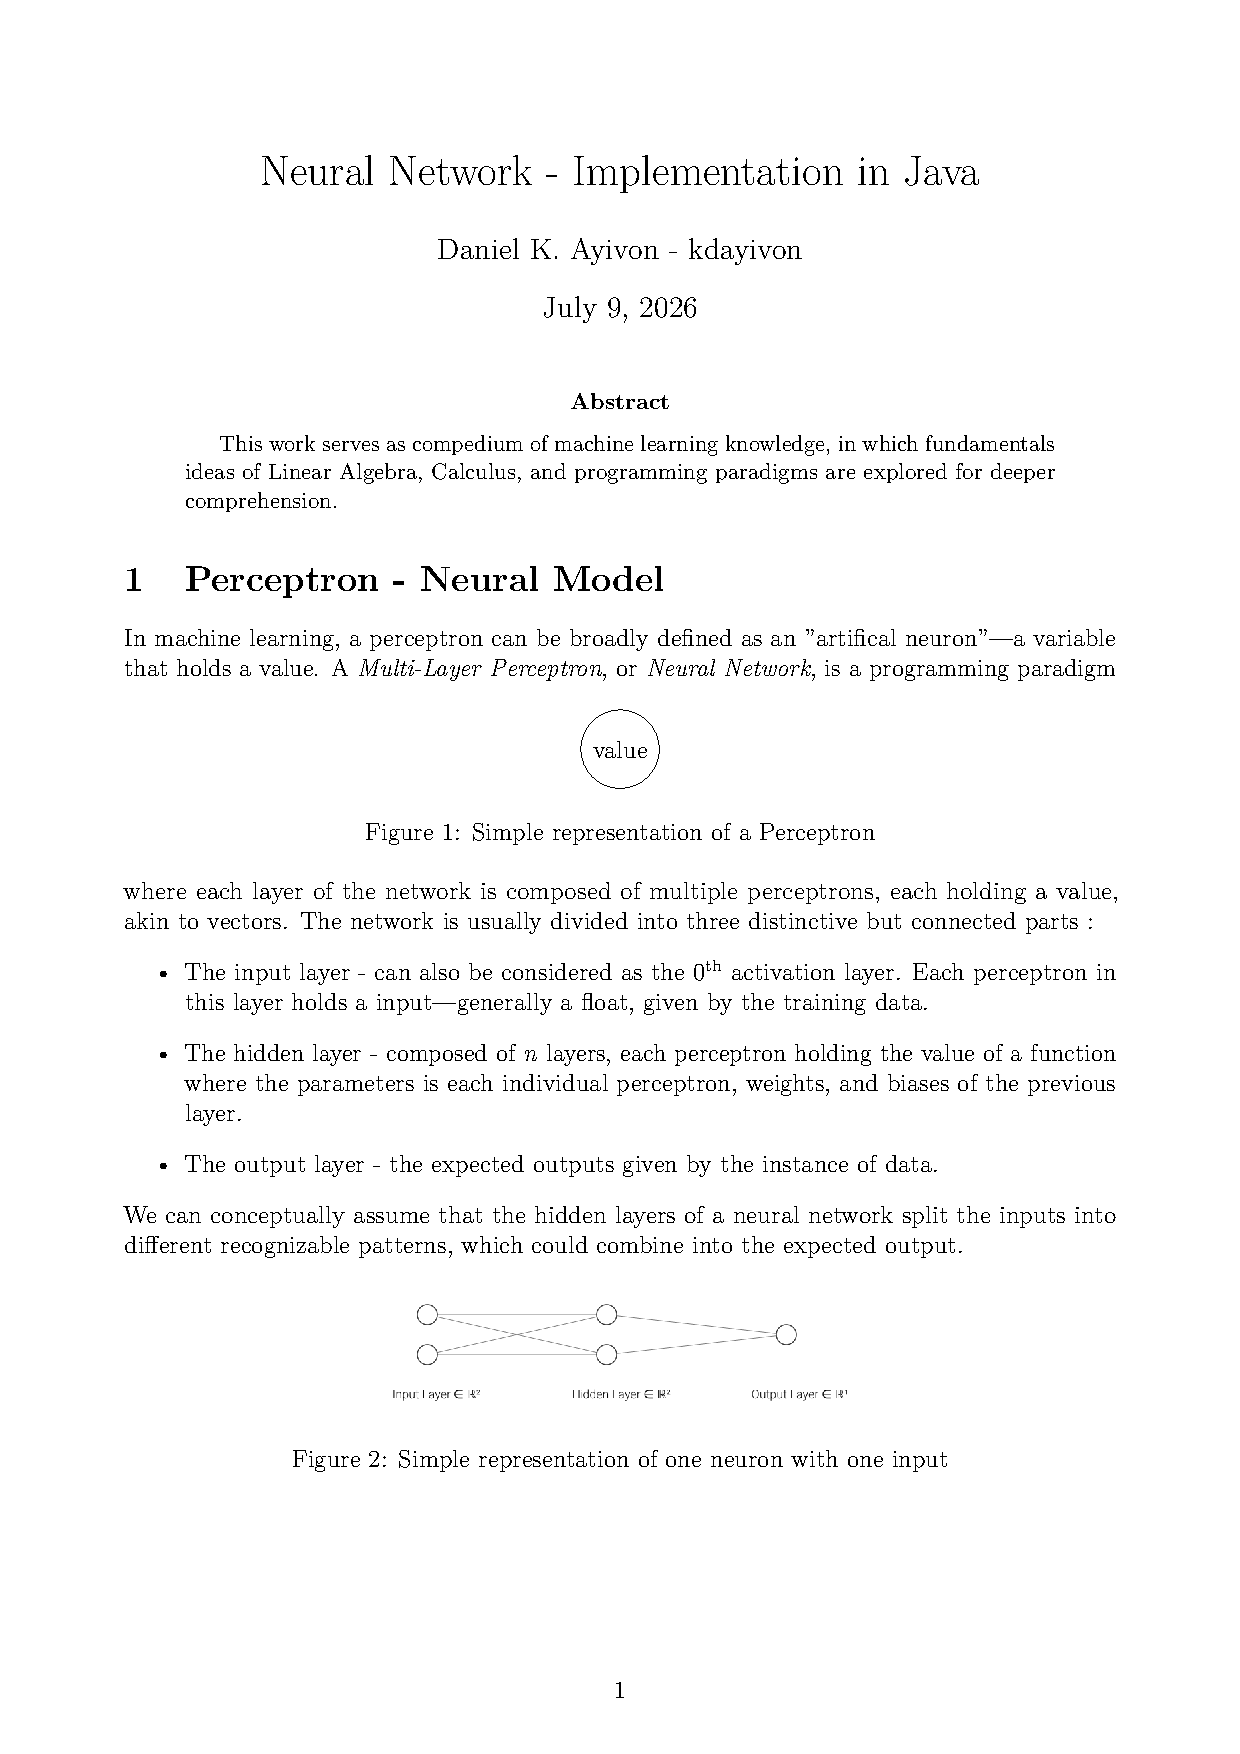
\includegraphics[width=0.5\textwidth]{nn.png}
        \caption{Simple representation of one neuron with one input}
        \label{fig:1n1i}
    \end{figure}
    \subsection{Forwarding} 
    The notion of \textit{forwarding} in an artificial neural network, is the process of sending information through the layers,
    from one layer to the next without forming loops or cycles. 
    In a forward-feeding network, each perceptron in the next layer is a function of sum that adds up all the perceptron in the
    layer before it (1)
    \begin{align} 
        \sum_{i = 1}^{n} w_{i}a_{i} 
    \end{align}
    where \textit{n} the number of perceptron in the previous layer, \textit{w} the weights (or parameters) of the model, 
    \textit{a} the activations or inputs of the model.
    The function in its current state can return any value $k \in \mathbb{R}$, prompting the need to compress (or map) 
    the values between an acceptable range, using functions known as \textit{activation functions}. The most common 
    activation functions are the \textbf{Sigmoid} and \textbf{ReLU} (Rectified Linear Unit) functions.
    \begin{align*} 
        \sigma(x) &= \frac{1}{1 - e^{-x}} \tag{Sigmoid function} \\ 
        ReLU(x) = \frac{x + |x|}{2} &=
        \left\{
            \begin{aligned}
                &x &\text{if } x > 0 \\
                &0 &x \le 0
            \end{aligned}
        \right.
        \tag{ReLU function}
    \end{align*}
    The final activation function (forwarding) is a measure of how positive the compressed value of this function is.
    
    \begin{align}
        k &= \sigma\left(\sum_{i=1}^{n} w_{i}a_{i} + b\right) \\
        k &= \sigma\left(
            \begin{bmatrix}
                w_{1,1} & w_{1,2} & \cdots & w_{1,n} \\
                w_{2,1} & w_{2,2} & \cdots & w_{2,n} \\
                \vdots  & \vdots  & \ddots & \vdots  \\
                w_{k,1} & w_{k,2} & \cdots & w_{k,n}
            \end{bmatrix}
            \begin{bmatrix}
                a_{1}^{0} \\ a_{2}^{0}\\ \vdots \\ a_{n}^{0} 
            \end{bmatrix}
            +
            \begin{bmatrix}
                b_{1} \\ b_{2} \\ \vdots \\ b_{k}
            \end{bmatrix}
        \right)
    \end{align}
    
    \section{Machine Learning}
    In \textit{Machine learning}, an elementary implementation of neural networks consists of finding an output $y$ 
    with a given input $x$, by adjusting different parameters in the equation
    \begin{align} 
        y &= xw + b
    \end{align}
    where $w$ is the weights, or connections between neurons, and $b$ is the bias where each neuron has its own. 
    For any random value given to the parameters, we must compute how different the output given by the equation and 
    the expected output is. 

    \subsection{Loss Function}
    In mathematical optimization and statistics, a \textit{loss function} is a function that maps values of one or more 
    parameters onto a real number that intuitively represents a "cost" associated with the event. It is used for parameter
    estimation, where the event is some function of the difference between the estimated and expected values for an instance 
    of data. The finite goal of elementary machine learning is to drive the value of "cost" or "lost" function towards zero.
    Calculus helps us find the minimum of such a function using different linear methods, referred to as "\textit{Gradient Descent}". 

    \subsubsection{Naive Implementation - Twice}
    In the primitive machine learning example \textit{Twice}, we computed the cost function as the sum of the square difference
    between the ouput of the model for each input and the expected output. 
    \begin{align} 
    C(w) &= \frac{1}{n}\sum_{i=1}^{n}(x_{i}w - y_{i})^2
    \end{align}
    If the value of the model (represented as $x_{i}w$) deviates too much from the expected value ($y_{i}$), squaring the difference 
    magnifies the error. We divide by the number of samples $n$, to compute the average cost over the entirety of the sample 
        

    \section{Numerical Gradients}
    The gradient of a function tells us the direction of steepest increase. In order to minimize the loss function, we compute the direction
    of the slope and move in the opposite. \textit{Numerical gradients}, as opposed to \textit{Analytical gradients}, are simple 
    conceptually and in implementation, but pose quite a challenge as the parameter count increases. Numerical gradients approximate 
    the derivative using discrete function values rather than analytical calculus, primarly via the \textbf{Finite Difference} methods, where 
    choosing an erroneous step size $h$ introduces numerical instability and precision issues. 
    Numerical Gradients work by applying a small perturbation to the parameters and observing how much the function value changes. 
    \begin{figure}[H]
        \centering
        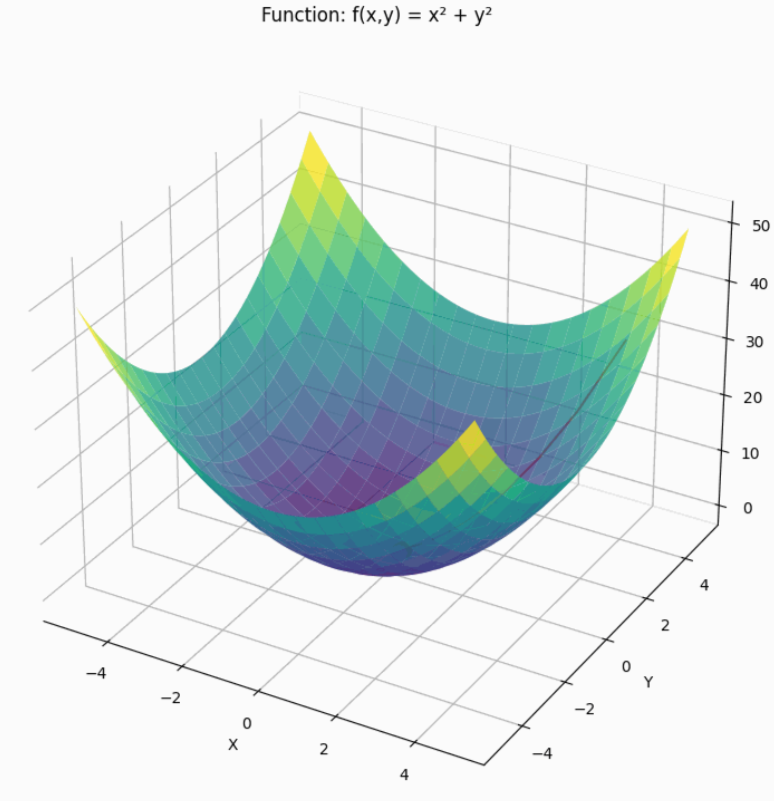
\includegraphics[width=0.5\textwidth]{numericaldescent.png}
        \caption{Gradient Descent - Numerical}
        \label{fig:nd}
    \end{figure}
    
    \subsection{Gradient Descent - Finite Difference}
    We use the finite difference to approximate the derivative of the function to hopefully find the global minimum; 
    Since we randomize the starting point of the function (by randomizing the values of the weights and biases), 
    there is a better chance to find a local minimum. As we arbitrarly choose a value that approaches 0 for the $\epsilon$, to
    help find the direction of the tangent to the curve. 
    \begin{align} 
        C(w) &= \frac{C(w + \epsilon) - C(w)}{\epsilon} 
    \end{align}
    
    \begin{align} 
        C'(w) &= \lim_{\epsilon \to 0}\frac{C(w + \epsilon) - C(w)}{\epsilon} 
    \end{align}

    \subsection{Faster Cost Compute}
    Essentially, instead of computing the cost function, seeing the value and adjusting the parameters and seeing if the cost 
    goes downward, we compute the velocity according to the value $w$, and keep subtracting from $w$ the derivative. This is 
    a faster and more accurate method as we don't need to specify a value that amounts to the step size down the function. We
    compute the derivative as the rule from calculus states 
    \begin{quote}
    If a function is differentiable, its minima occurs at points where the derivative is zero. 
    \end{quote}

    \begin{align} 
        C(w) &= \frac{1}{n}\sum_{i=1}^{n}(x_{i}w - y_{i})^{2} \\ 
        C'(w) &= \left(\frac{1}{n}\sum_{i=1}^{n}(x_{i}w - y_{i})^{2}\right)' = \\ 
        &= \frac{1}{n}\left(\sum_{i=1}^{n}(x_{i}w - y_{i})^{2}\right)' \\ 
        &= \frac{2}{n}\sum_{i=1}^{n}(x_{i}w - y_{i})x_{i} \\ 
    \end{align} 

    As we're taking the derivative of a smooth quadratic function, it possesses a single global minimum where the derivative 
    is null. The function also needs to be convex, meaning it needs to be twice-differentiable with its second derivative 
    being nonnegative on its entire domain. 
    \begin{align} 
        C"(w) &=\frac{2}{n}\sum_{i=1}^{n}x_{i}^{2} > 0
    \end{align}
    The difference between this gradient descent algorithm and computing the fintite difference, is that the model becomes
    too sensitive to the value $\epsilon$ we manually specified, making it hard to land on a specific value if the $\epsilon$
    value is too big. 

    \section{Analytical Gradient}
    


    \subsection{neuron}
    \begin{figure}[htbp]
        \centering
        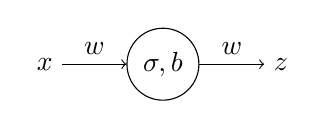
\begin{tikzpicture}
            \def\d{1.5}
            \node (X) at (-\d, 0) {$x$};
            \node[shape=circle, draw=black] (N) at (0, 0) {$\sigma, b$}; 
            \node (Y) at (\d, 0) {$z$};
            \path[->] (X) edge node[above] {$w$} (N);
            \path[->] (N) edge node[above] {$w$} (Y);
        \end{tikzpicture}
        \caption{Simple representation of a Perceptron}
        \label{fig:n1i}
    \end{figure}
\end{document}
